
\item \points{90} {\bf Учење подстицајем: обрнуто клатно}

У овом задатку биће примењено учење подстицајем да се аутоматски одреди политика за релативно сложен управљачки проблем без залажења у појединости динамике система којим се управља.

Задатак који ће бити размотрен је такозвани проблем обрнутог клатна или балансирања стуба.\footnote{Динамика је преузета са {\tt https://all.cs.umass.edu/rlr/domains.html}}

Размотрити приказану слику. Танак стуб је преко шарке повезан са колицима која се могу кретати латерално по глаткој површини стола. Каже се да је контролер отказао ако угао стуба одступа више од одређене границе у односу на вертикални положај, то јест ако је стуб пао или ако положај колица изађе ван оквира, то јест ако падну са ивице стола. Циљ је развити контролер који балансира стубом унутар ових ограничења тако што ће колица на одговарајући начин убрзавати лево и десно.

\begin{center}
 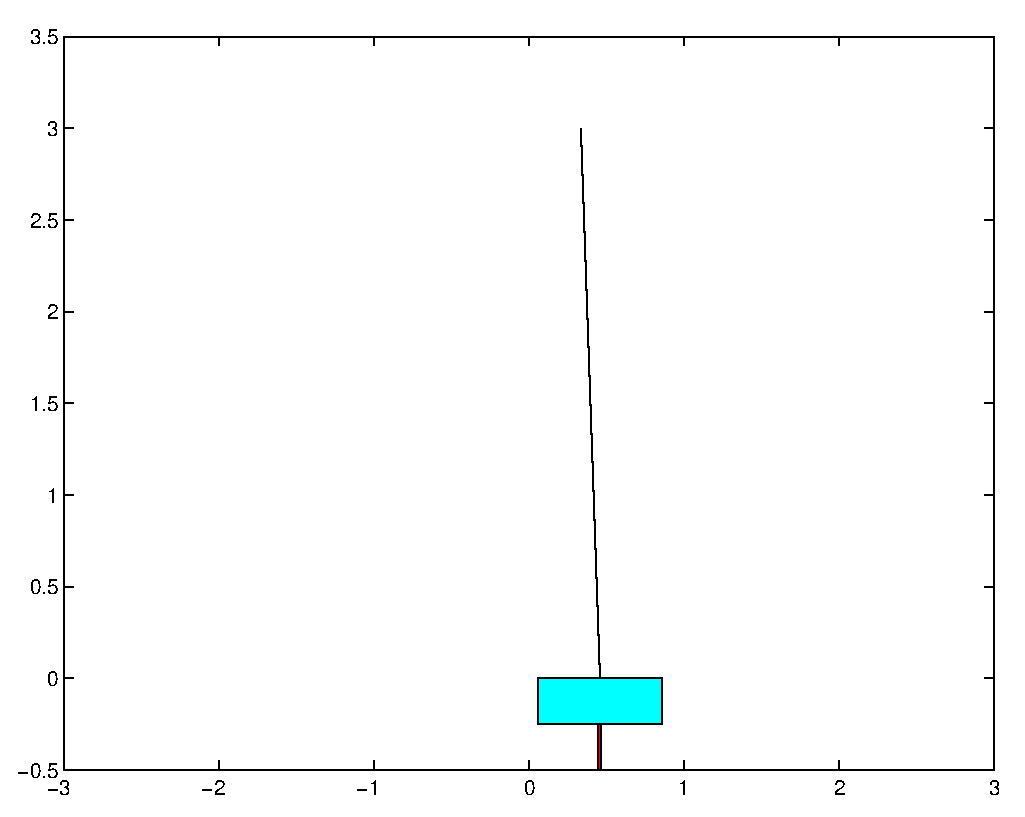
\includegraphics[width=6cm]{cartpole/cart_pole.eps}
\end{center}

За овај задатак направљен је једноставан симулатор. Симулација се одвија у дискретним временским корацима. Стање колица и стуба у било ком тренутку у потпуности одређују четири параметра: положај колица $x$, брзина колица $\dot{x}$, угао стуба $\theta$ мерен као његово одступање од вертикалног положаја, као и угаона брзина стуба $\dot{\theta}$. Пошто је једноставније разматрати учење подстицајем у дискретном простору стања, простор стања је апроксимиран дискретизацијом која пресликава вектор стања $(x,\dot{x}, \theta, \dot{\theta})$ у број од 0 до {\tt NUM\_STATES-1}. Стога ће алгоритам учења подстицајем радити само над овом дискретном представом стања.

У сваком тренутку у времену, односно временском кораку, контролер мора изабрати једну од две акције - гурнути (убрзати) колица удесно или гурнути (убрзати) колица улево. (Да би се задатак у потпуности поједноставио, не постоји {\it не ради ништа} акција.) Претходне две акције су у изворном коду представљене са $0$ и $1$, респективно. Када се изабере једна од две акције, симулатор ажурира параметре стања у складу са динамиком система и враћа ново дискретизовано стање.

Биће усвојена претпоставка да је награда $R(s)$ функција само тренутног стања. Када угао стуба пређе одређену границу или када колица оду предалеко, додељује се негативна награда, а систем се поново иницијализује у случајно почетно стање. Иначе, у сваком другом тренутку, награда је нула. Програм мора научити да балансира стуб користећи само опажане односно посматране прелазе стања и награде.

Датотеке за овај задатак се налазе у {\tt src/cartpole/} директоријуму. Већина кода је већ написана, а потребно је само допунити {\tt cartpole.py} датотеку на назначеним местима. Ова датотека може се покренути како би се добио графички приказ и како би се на крају исцртале криве учења. За више детаља о раду симулатора прочитати коментаре у заглављу датотеке.

Да би се решио задатак обрнутог клатна, неопходно је најпре проценити модел (односно, вероватноће прелаза и награде) за Марковљев поступак одлучивања (МПО) који је у основи проблема, затим решити Белманове једначине за тако процењен МПО да би се добила функција вредности, и најзад, деловати похлепно у односу на ту функцију вредности.

Укратко, биће одржаван тренутни модел МПО и тренутна процена функције вредности. У почетном тренутку, свако стање има процењену награду нула, а процењене вероватноће прелаза су униформне (подједнако је вероватно да се заврши у било ком другом стању).

Током симулације, у сваком временском тренутку морају се изабрати акције у складу са неком тренутном политиком. Како програм буде напредовао у извршавању радњи, прикупљаће запажања о преласцима и наградама које може искористити за бољу процену МПО модела. Пошто је крајње неефикасно ажурирати цео процењени МПО након сваког посматрања, опажања о променама стања и наградама биће чувана у сваком кораку, а модел и функција вредности, односно политика ће бити ажурирани само периодично. Стога је неопходно чувати укупан број опажених прелазака из стања $s_i$ у стање $s_j$ користећи акцију $a$ , а слично томе и за награде. Треба имати у виду да су награде у било ком стању детерминистичке, али промене стања услед дискретизације простора стања нису (неколико блиских, али различитих конфигурација се могу пресликати у једно те исто дискретизовано стање).

Сваки пут када дође до отказа (на пример, ако стуб падне или колица оду ван стола), требало би поново да се процене вероватноће прелаза и награде као просек посматраних врености (ако их уопште има). Програм тада мора користити итерацију по вредности да реши Белманове једначине на процењеном МПО како би добио функцију вредности и нову оптималну политику за нови модел. За итерацију по вредности треба користити критеријум конвергенције који проверава да ли максимална апсолутна промена функције вредности у некој итерацији премашује одређену унапред задату толеранцију.

Коначно, претпоставити да је целокупан поступак учења конвергирао када сваки од неколико узастопних покушаја (дефинисаних параметром {\tt NO\_LEARNING\_THRESHOLD}) решавања Белманових једначина конвергира у првој итерацији. Интуитивно, ово указује да је процењени модел престао да се значајно мења.

Нацрт изворног кода за овај задатак се већ налази у {\tt cartpole.py} и потребно је само дописати делове кода у назначеним местима унутар датотеке. Постоји и неколико додатних појединости (критеријуми конвергенције и слично) који су такође додатно појашњени унутар самог изворног кода. Користити фактор попуста $\gamma = 0.995$.

Имплементирати алгоритам учења подстицајем као што је наведено и покренути га.

\begin{itemize}
\item Колико покушаја (односно колико пута су стуб или колица пали) је било потребно пре него што је алгоритам конвергирао? Смерница: у тачном решењу, на графику који представља логаритам усредњеног броја корака до отказа, црвена линија треба да почне да се заравњује након шездесетак итерација.

\item Нацртати криву учења која приказује број временских корака за коју је стуб балансиран за сваку симулацију. Укључити график у извештај.
  
\item Променити {\tt np.random.seed} на вредности вредностима 1, 2 и 3 и поново покренути програм. Која су запажања? Шта ово говори о самом алгоритму?
\end{itemize}

\ifnum\solutions=1 {
  \begin{answer}
\end{answer}

} \fi
